\documentclass{article}

\usepackage[pdftex]{graphicx}

\usepackage{svg}
\usepackage{listings}
\usepackage{color}
\usepackage{times}
\usepackage{amsfonts}
\usepackage{draftwatermark}
\usepackage{hyperref}
\usepackage{algorithm}
\usepackage{algorithmic}
\SetWatermarkText{DRAFT}
\SetWatermarkScale{1}
\SetWatermarkLightness{0.95}

\lstset{
float, 
mathescape=true, 
texcl=true,
basicstyle=\footnotesize\ttfamily,
columns=fixed,
numbers=none,%left,
stepnumber=1,
captionpos=b,
showstringspaces=true,
language=C++,
keywordstyle=\color[rgb]{0.0, 0.0, 0.8},
stringstyle=\color[rgb]{0.5, 0.0, 0.5},
tabsize=4,
commentstyle=\color[rgb]{0.133,0.545,0.133}\textit,
morekeywords={ },
frame=single,
}

\begin{document}

\title{Dynamic AABB Trees}
\author{Erin Catto\\Blizzard Entertainment}
\maketitle

\begin{figure}
	\begin{center}
	\end{center}
	\includesvg[width=0.6\textwidth]{images/Rotate}
	\caption{A tree rotation that can be used to mitigate a degenerate BVH.}
	\label{fig:teaser}
\end{figure}

\begin{abstract}
\small
This document presents techniques for using dynamic AABB trees in games. The surface area heuristic is used as the cost metric for tree insertions. An efficient branch and bound search is used to find the globally best insertion location. Tree rotations are used to prevent poorly formed trees in the case of sorted input, which is typical in authoring tools and procedural generation of game environments.
\end{abstract}

\section{Introduction}
Physics engines for games usually have a \emph{broad-phase} to accelerate ray casts, shape casts, and overlap tests. Typically there are many dynamic objects and a static environment. Furthermore, steaming environments need to load and unload both static and dynamic objects without pausing the game for a load screen.

For simple games, a brute force approach with an array of axis-aligned bounding boxes (AABBs) can suffice. Once there are more than 20 or so objects, a better acceleration structure can improve performance. 

There are other data structures that work for dynamic environments. The two main data structures used in modern physics engines are the sweep-and-prune \cite{Bergen2004} and dynamic AABB trees \cite{Presson2008}. Sweep-and-prune data structure has fallen out of favor due to poor scaling for long ray casts in large worlds.

This leaves the dynamic AABB tree as the favorite among many of the physics engines in active development. There are a number of techniques that can be applied to an AABB tree to make it suitable for dynamic worlds. These will be covered in the following sections.

The AABB tree is specific type of bounding volume hierarchy (BVH). The AABB is the bounding volume and the hierarchy is a binary tree. Other choices are possible, such as bounding spheres and K-DOPs. On modern SIMD hardware the AABB is a simple and efficient shape. Further, an $n$-ary tree is possible, but a binary tree is easy to implement and yields efficient data structures.

The AABB tree supports several queries efficiently: ray-casts, sphere-casts, general shape-casts, and AABB overlap queries. AABB trees can also support efficient closest point queries using a branch and bound algorithm.

This article covers the incremental construction of AABB trees suitable for games. Games need to handle dynamic updates to the tree as objects move. Objects in games are often created and destroyed in real-time. When a game is loading it is beneficial to build the AABB tree incrementally to spread out the cost across several frames. Finally, games often have streaming worlds where objects are loaded and unloaded as the player traverses the world.

The \emph{Surface Area Heuristic} and \emph{branch and bound} are used to build the tree incrementally. This leads to high quality trees in many cases. Object movement is handled be removing and re-inserting leaf nodes from the tree. Temporal coherence is used to avoid tree leaf re-insertion by using enlarged AABBs in the tree.

Sorted input is a common problem in games where procedural general will place many similar objects sequentially. Such scenarios can lead to degenerate AABB trees that take the form of linked lists. This has the impact of making queries take $O(N)$ time instead of the typical $O(log N)$ time associated with binary trees. Using tree rotations during the insertion process is shown to mitigate this effect.

\section{Related Work}
Much of the recent research on bounding volume hierarchies comes from the ray tracing community. While ray casting performance is clearly critical in ray tracing, it is also important in games. Especially games with a client-server architecture like Overwatch, where the server performs all gameplay logic and must therefore perform many ray casts. The cost of these ray casts directly influences the server scalability and the cost of hosting the game.

Often bounding volume hierarchies are compared with kd-trees. Generally kd-trees are faster, but take longer to build and use more memory~\cite{Vinkler2014}. On the other hand, BVHs can more readily handle dynamic scenes be they are object rather than spatially based.

Early work on bounding volume hierarchies focused on moving from manual to automatic construction. Goldsmith and Salmon~\cite{Goldsmith1987} developed the notion of the \emph{Surface Area Heuristic} and used it to build bounding volume hierarchies. Omuhundrol~\cite{Omohundrol1989} (TODO ERIN).

Later authors began to consider handling dynamic hierarchies. Bergen~\cite{Bergen1998} built AABB trees using a top down build with mid-point splits and handled movement using refitting. Larson and Möller~\cite{Larsson2006} also used a top down mid-point split build with refitting, but added lazy sub-tree rebuilding.

Soon authors began to use tree re-configuration operations to improve the BVH. Otaduy et al~\cite{Otaduy2007} used a top down build with mid-point splits. They introduced AVL style tree rotation operations to keep the tree balanced. They also used a grand-children shuffling operation to optimize a squared volume heuristic. Kensler~\cite{Kensler2008} used hill climbing and simulated annealing to apply tree rotations to optimize the surface area heuristic. Kopta and Kensler~\cite{Kopta2012} applied refitting and rotations accross the whole tree after each frame of animation. Bittner et al~\cite{Bittner2013} used node removal and re-insertion to optimize existing trees using the SAH.

Bittner et al~\cite{Bittner2015} and Presson~\cite{Presson2008} developed incremental construction algorithms. Bittner used the SAH and branch and bound, while Presson used the Manhattan norm between AABB centers.

\section{Incremental Tree Construction}

Dynamic trees need to support the efficient insertion and removal of leaf nodes. The key operation is insertion. Games need to build large trees quickly that provide fast queries.

Consider the binary tree of Figure~\ref{fig:example_tree}. Adding a new leaf node $L$ to the tree is broken up into 3 stages:
\begin{enumerate}
	\item[Stage 1] Identify a sibling $S$ for $L$. This can be an existing internal node or leaf node.
	\item[Stage 2] Disconnect $S$ from the tree and create a new internal node $P$ in place of $S$. Make $S$ and $L$ children of $P$.
	\item[Stage 3] Refit the AABBs of the ancestors of $P$.
\end{enumerate}

\begin{figure}
	\begin{center}
		\includesvg[pretex=\large, width=\textwidth]{images/ExampleBinaryTree}
	\end{center}
	\caption{Example binary tree}
	\label{fig:example_tree}
\end{figure}

The Surface Area Heuristic is used to guide Stage 1. All nodes can be a sibling. The sibling is chosen that yields the small surface area increase. The increased surface area for a given sibling is due the creation of a new internal node and the increase surface area of the ancestors.

Figure~\ref{fig:insert_leaf} shows $L$ inserted with $H$ as the sibling. Node $11$ is the new internal node. The surface area increase to the tree is the surface area the new node plus the increased area of the ancestors of $L$:
\begin{equation}
	C_H = SA(11) + \Delta SA(10) + \Delta SA(8) + \Delta SA(7) + \Delta SA(3) + \Delta SA(1)
\end{equation}
The increased surface area of a node $i$ is:
\begin{equation}
	\Delta SA(i) = SA(i \cup L) - SA(i)
\end{equation}
In general the cost of any sibling $S$ choice is the area of the new internal node $P$ plus the increased area of the ancestors. The area of the $P$ is called the \emph{direct cost} and the increased area of the ancestors is the \emph{inherited cost}.
\[ C_S = SA(P) + \sum_{i \in ancestors(P)} \Delta SA(i) \]
Note that the area of $L$ is not included the cost function because only the relative cost matters when considering potential siblings for $L$.

\begin{figure}
	\begin{center}
		\includesvg[pretex=\large, width=\textwidth]{images/TreeInsert2}
	\end{center}
	\caption{Inserting new leaf $L$ into tree with new parent node $11$}
	\label{fig:insert_leaf}
\end{figure}

For a binary tree with $N$ leaf nodes, there are $2N - 1$ possible siblings. Finding the best sibling by visiting every node and computing the increased surface area is quite expensive, especially during the initial construction of the tree.

The \emph{branch and bound} algorithm can be used to accelerate the search for the best sibling. Brand and bound is a recursive algorithm like depth-first search or bread-first search. Instead of using a stack or a queue, branch and bound uses a priority queue, which can be implemented as a min-heap.

As describe by Bittner~\cite{Bittner2013}, branch and bound uses a priority queue to find the best sibling. The branch and bound algorithm requires a lower bound estimate for the cost for a subtree. A lower bound on the cost for any node and the sub-tree below is:
\begin{equation}
	C_{lower} = SA(L) + C_I
\end{equation}
where
\begin{equation}
	C_I = \sum_{i \in ancestors(S)} \Delta SA(i)
\end{equation}
In this case the direct cost is just the surface area of $L$. This represents the smallest possible parent for $L$ and a sibling. The ancestor cost is what makes the lower bound effective.

The branch and bound algorithm starts by computing the cost of root node:
\[ C_{root} = SA(root \cup L) \]
This is set as the best cost, \[C_{best} = C_{root} \] and as the best sibling, \[S_{best} = root\]. The root node is pushed onto the priority queue along with the inherited cost of the root node, which is $0$.

\begin{algorithm}
	\caption{Find best sibling for $L$}
	\label{alg:best_sibling}
	\begin{algorithmic}
		\STATE $S_{best} = root$;
		\STATE $C_{best} = SA(L \cup root)$
		\STATE push($Q$, [$root$, $\Delta SA(root)$])
		\WHILE{$Q$ is not empty}
		\STATE [$S$, $C_I$] = pop($Q$)
		\STATE $C_{lower} = C_I + SA(L)$
		\IF{$C_{lower} >= C_{best}$}
		\RETURN $S_{best}$
		\ENDIF
		\FORALL{children $k$ of $S$}
		\STATE $C_k = SA(S_k \cup L) + C_I$
		\IF{$C_k < C_{best}$}
		\STATE $C_{best} = C_k$
		\STATE $S_{best} = S_k$
		\ENDIF
		\STATE $C_I = C_k - SA(S_k)$
		\IF{$C_I + SA(L) < C_{best}$}
		\STATE push($Q$, [$S_k$, $C_I$])
		\ENDIF
		\ENDFOR
		\ENDWHILE
	\RETURN $S_{best}$
	\end{algorithmic}
\end{algorithm}

\section{Object Movement}

Game objects often need to be created and destroyed at run time due to game logic. Also simulated and animated objects need to move. There are several techniques for adapting a BVH to movement.
\begin{enumerate}
	\item Refit ancestors
	\item Rebuild subtrees
	\item Leaf re-insertion
\end{enumerate}
Refitting ancestors is typically a quick $O(log N)$ operation. However, if an object moves a long distance the quality of the tree can degrade. Rebuilding sub-trees~\cite{Larsson2006} has up to $O( N log N )$ cost depending on the location of the root. For a high frame rate game, this is likely too expensive. Leaf re-insertion usually has $O(log N)$ cost and can improve the quality of the tree. Additionally it uses the same algorithms needed to handle object creation and destruction.

The frequency of leaf re-insertion can be reduced in many game. Often objects do not move far per frame in a game, especially if the frame rate is over 30 Hertz. Using this notion of \emph{temporal coherance} we can enlarge the bounding box used in the tree for moving objects. Each time an object moves, the code checks to see if the object's tight fitting bounding box is fully contained in the enlarged bounding box. If the tight bounding box is fully contained then leaf re-insertion is not needed. This can greatly reduce the number of leaf re-insertions on average.

Here are some heuristics for bounding box enlargement.
\begin{enumerate}
	\item Fixed increase
	\item Relative increase
	\item Predictive increase
\end{enumerate}
The fixed increase simply adds a fixed offset to the AABB extents in all dimensions. The relative increase uses an extend offset that scales with the object size. A predictive increase uses the object's velocity to enlarge the AABB in the direction of movement. All of these heuristics can be combined.
The best choice can depend on the type of game and the object movement patterns. It is worth mentioning that predictive increase can be risky because it may leaf an excessively large AABB in the tree even after the object starts moving. It may make sense to re-insert the object when it comes to rest using a smaller AABB.

\section{Sorted Input}
Goldsmith~\cite{Goldsmith1987} noted that sorted input is problematic in tree construction. In games sorted input is often unavoidable. Voxel style worlds in 3D and tile-base worlds in 2D are easy examples. Procedurally generated game worlds are likely to have objects that are sorted. Even when game worlds are manually created, object duplication may result in areas that are at least locally sorted and uniform.

For example, consider the ordered objects in Figure~\ref{fig:tile_based}. When these objects are inserted into an empty tree in order from left to right, then a tree is built as shown in Figure~\ref{fig:linked_list}. Even though the SAH optimal choice is made for each leaf insertion, the final tree is far from optimal. In this case the optimimal tree should be balanced. Instead the tree has the form a of linked list. This makes ray casts take $O(N)$ time.

\begin{figure}
	\begin{center}
		\includesvg[pretex=\Large]{images/TileBased}
	\end{center}
	\caption{Sorted input of a tile-based world common in 2D games.}
	\label{fig:tile_based}
\end{figure}

\begin{figure}
	\begin{center}
		\includesvg[pretex=\Large]{images/LinkedList}
	\end{center}
	\caption{Tree built in the shape of a linked list.}
	\label{fig:linked_list}
\end{figure}

The linked list tree structure also particularly troubling because this causes large stack usage in recursive ray-cast algorithms. If a local stack is used, this can lead to heap allocations which can further cripple performance. One is better off using a brute-force algorithm.

\section{Tree Rotations}
Tree rotations were applied by Kensler~\cite{Kensler2008} to optimize a tree after it is built. These are local operations similar to AVL and red-black tree rotations. Unlike traditional binary trees used for sorting, bounding volume hierarchies do not require child ordering. For example, Figure~\ref{fig:equivalent_trees} shows two binary trees that are equivalent bounding volume hierarchies.

\begin{figure}
	\begin{center}
		\includesvg[pretex=\tiny, width=\textwidth]{images/EquivalentTrees}
	\end{center}
	\caption{Equivalent bounding volume hierarchies}
	\label{fig:equivalent_trees}
\end{figure}

Figure~\ref{fig:possible_rotations} shows four possible sub-tree rotations when a node has four grandchildren. As Kensler noted, only the child areas of $B$ and $C$ can change after rotation. The bounding box of the sub-tree root $A$ does not change, nor do the bounding boxes of the grandchildren $D$, $E$, $F$, and $G$. Thus this is a local operation that can be applied to any sub-tree inside a binary tree, as long as the sub-tree root has grandchildren. In the case where the sub-tree root has only two grandchildren, two possible rotations exist.

\begin{figure}
	\begin{center}
		\includesvg[pretex=\large, width=0.8\textwidth]{images/RotatePossible}
	\end{center}
	\caption{Four possible tree rotations. Each rotation swaps a child node with a grandchild node.}
	\label{fig:possible_rotations}
\end{figure}

Tree rotations can be applied to deal with sorted input. In Stage 3 of leaf insertion the ancestor bounding boxes are refitted to contain the new leaf. Immediately after an ancestor is refitted the four possible rotations are considered. If a lower total surface area for the children $B$ and $C$ is found the rotation is performed. Then the refitting process continues until the root node is reached. This process is illustrated in Algorithm~\ref{alg:stage3}. For brevity the actual rotation operation is left out since it is just a simple (but somewhat lengthy) matter of re-arranging indices and updating the bounding box of $B$ or $C$. Also the algorithm assumes $B$ and $C$ are both internal nodes. The algorithm can be easily adapted to the case of $B$ or $C$ being a leaf node (but not both).

\begin{algorithm}
	\caption{Stage 3: Refit tree after inserting $L$. Assumes $B$ and $C$ are internal nodes at each level.}
	\label{alg:stage3}
	\begin{algorithmic}
		\STATE $P = parent(L)$
		\STATE $A = parent(P)$
		\WHILE{$A$ is not null}
		\STATE \COMMENT{Refit $A$}
		\STATE $A = B \cup C$ 
		\STATE \COMMENT{Compute rotation costs}
		\STATE $C_{base} = SA(B) + SA(C)$
		\STATE $C_{BF} = SA(B) + SA(B \cup G)$
		\STATE $C_{BG} = SA(B) + SA(B \cup F)$
		\STATE $C_{CD} = SA(C) + SA(C \cup E)$
		\STATE $C_{CE} = SA(C) + SA(C \cup D)$
		\STATE Perform best rotation \COMMENT{omitted for brevity}
		\STATE $A = parent(A)$
		\ENDWHILE
	\end{algorithmic}
\end{algorithm}

\section{Results}
Results are generated using the open source library \emph{dynamic-tree}~\cite{Catto2019}.

Results are compared using the \emph{surface area ratio} (SAR). This is a non-dimensional number that compares the area of the internal nodes to the area of the root node. Let $T$ be the set of internal nodes excluding the root node, then:
\begin{equation}
	SAR = \frac{\sum_{i \in T} SA(i)}{SA(root)}
\end{equation}

Algorithm~\ref{alg:stage3} produces a balanced binary tree for sorted input. The input of Figure~\ref{fig:tile_based} produces the tree shown in Figure~\ref{fig:sort_balanced}.

\begin{figure}
	\begin{center}
		\includesvg[pretex=\small, width=0.8\textwidth]{images/sort_balanced}
	\end{center}
	\caption{Balanced tree produced using tree rotations during the refit phase of leaf insertion.}
	\label{fig:sort_balanced}
\end{figure}

\section{Conclusion}

\section{Subtree Rotations}

Consider a game world with many identical geometric objects in a row as shown in Figure~\ref{fig:tile_based}. Such configurations are common in games, especially in tile-based or voxel-based game worlds. The dynamic tree is built by inserting objects from left to right. The resulting tree is shown in Figure~\ref{fig:linked_list}. This is an undesirable tree because it is has the form of a linked list and the height of the tree is equal to the number of objects. Using an area of 1 for the AABB of each game object, the tree a total internal node area of 35. A balanced tree shown in Figure~\ref{fig:balanced} has a total internal node area of 24.

\begin{figure}
	\begin{center}
		\includesvg[pretex=\Large]{images/Balanced}
	\end{center}
	\caption{Balanced tree. The area is shown next to each internal node. Total internal node area is 24. }
	\label{fig:balanced}
\end{figure}

How does the insertion algorithm generate such a poor tree? The answer is seen by looking at the insertion algorithm. The nodes are inserted in spatial order and the tree is making the same cost analysis for each new leaf. This causes the tree to grow down one side. The insertion algorithm is unable to restructure the tree to achieve a balanced structure. This sensitivity to ordered data was recognized by Goldsmith~\cite{Goldsmith1987}.

In a game environment typically the tree is initially built when the game is loaded. Then the tree needs to handle movement of a varying subset of the world as well as occasional addition and removal of objects. The initial build of the tree is the most critical time. The tree needs to be filled quickly and needs to have reasonable performance. It must tolerate ordered insertions.

Consider a subtree rotation as shown in Figure~\ref{fig:rotate}. In this rotation, subtree $B$ is swapped with $F$. There are three other rotations possible: $B \Leftrightarrow G$, $C \Leftrightarrow D$, and $C \Leftrightarrow E$. These rotations in subtrees that contain three levels. It is possible that $B$ or $C$ are leaf nodes. If $B$ is a leaf, then valid rotations are restricted to $B \Leftrightarrow F$ and $B \Leftrightarrow G$. If $C$ is a leaf then $C \Leftrightarrow D$ and $C \Leftrightarrow E$ are valid. These operations are do not change the AABB for node $A$.

\begin{figure}
	\begin{center}
		\includesvg[pretex=\Large, width=\textwidth]{images/Rotate}
	\end{center}
	\caption{Tree rotation, $B \Leftrightarrow F$ }
	\label{fig:rotate}
\end{figure}

These rotation operations can be used to optimize the surface area of $B$ and $C$. For example, the rotation $B \Leftrightarrow F$ shown in Figure~\ref{fig:rotate} can be used to reduce the surface area of $C$. The choice of rotation is made against the base cost of $B$ and $C$:
\[ C_{BC} = SA(B) + SA(C) \]
For the rotation $B \Leftrightarrow F$ the cost is:
\[ C_{BF} = SA(B) + SA(B \cup G) \]
There are similar formulas for the other rotations. There are a total of 5 possibilities: the base case and the four rotations.

Rotations are introduced to the insertion algorithm in Stage 3. While ascending the tree, rotations are applied at each node that has two levels below (has grandchildren). This is done after the node's height and AABB are updated.

Using the modified Stage 3 with rotations applied to the case of Figure~\ref{fig:tile_based} leads directly to the balanced tree of Figure~\ref{fig:balanced}.

\section{Object Movement}

Games must handle object movement in the tree. Refitting the AABBs is not a good strategy due to the typical large movement of game objects. Instead objects are removed from the tree and re-inserted when they move. 

Objects in a game world tend to move coherently and the distance per frame is often small relative to a their size. Therefore, objects use inflated AABBs in the tree. When an object moves, the actual AABB is compared with the inflated AABB. If the actual AABB is fully contained by the inflated AABB, then no tree update is necessary.

\begin{figure}
	\begin{center}
		\includesvg[pretex=\Large, width=0.25\textwidth]{images/InflatedAABBs}
	\end{center}
	\caption{Inflated AABBs (solid) allow actual AABBs (dashed) to move by some amount without requiring a tree update. }
	\label{fig:inflated}
\end{figure}

\section{Results}

A simple but non-trivial test was performed in Box2D using the scene from Figure~\ref{fig:pyramid}. The scene consists of 33 1-by-1 boxes. Since this is 2D, the perimeter is used by the surface area heuristic. So each box has an \emph{area} of 4. The boxes are created in order fashion, left to right, bottom to top.

\begin{figure}
	\begin{center}
		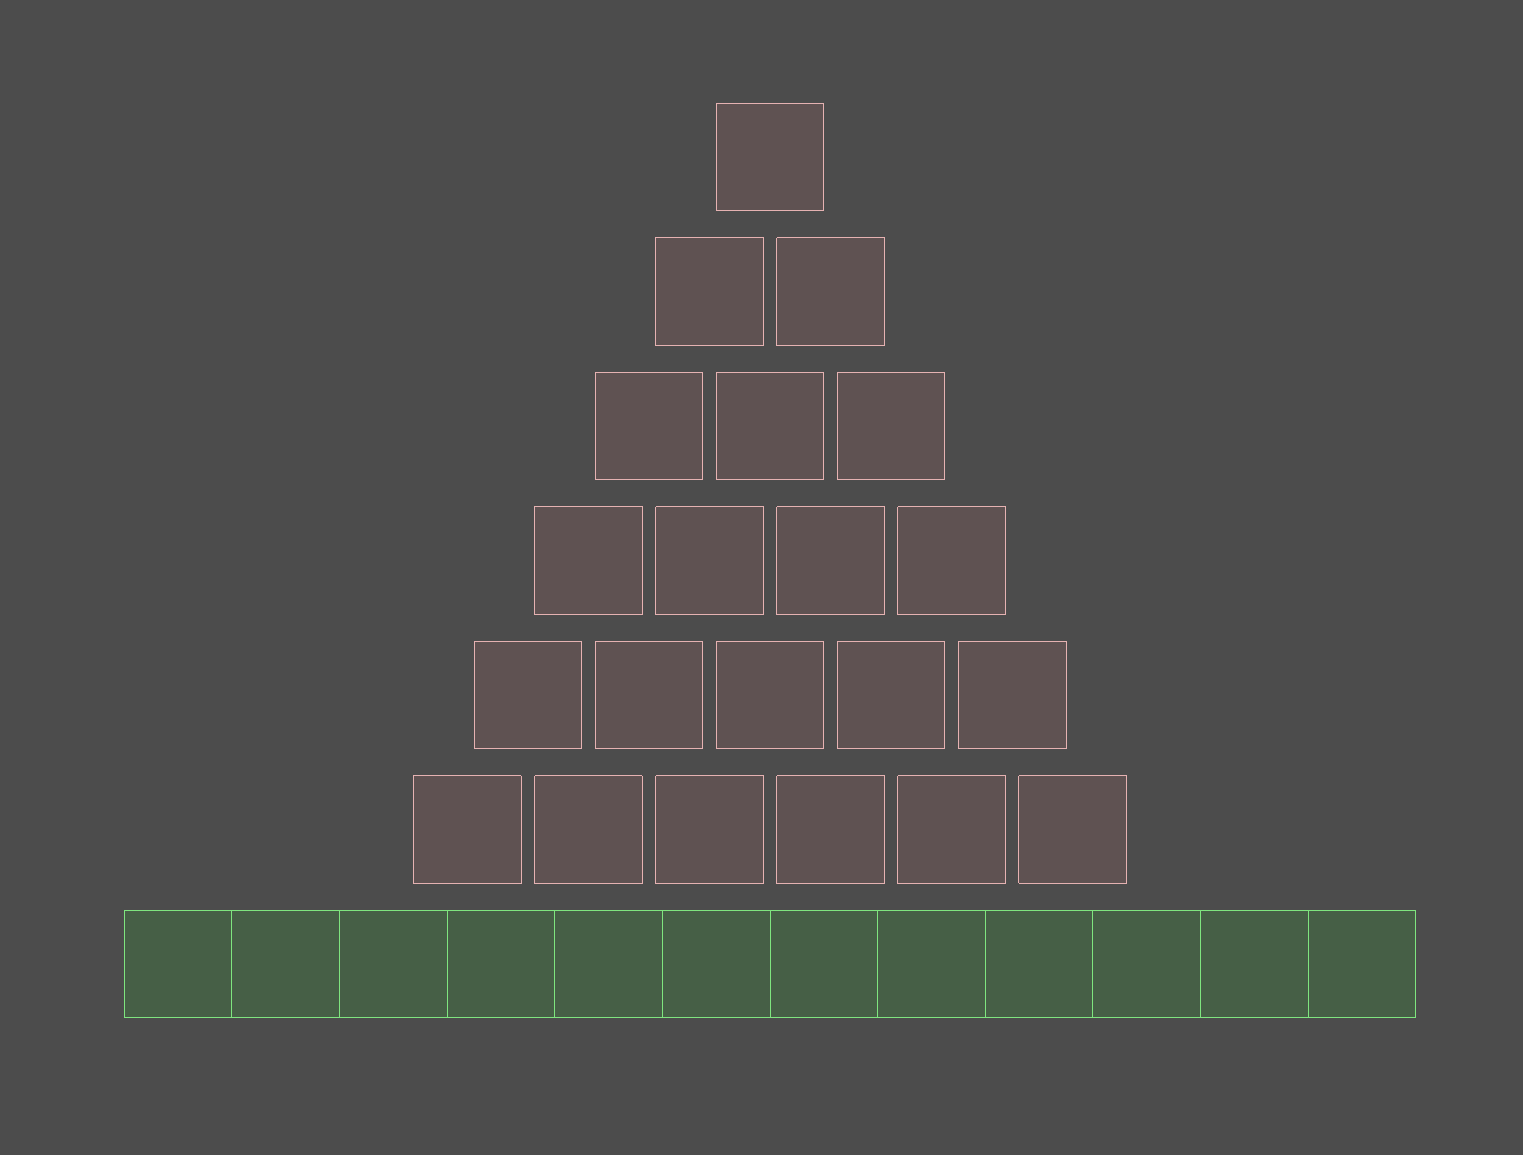
\includegraphics[width=0.5\textwidth]{images/Pyramid}
	\end{center}
	\caption{ Pyramid test from Box2D. Each box is 1-by-1 units (perimeter = 4).}
	\label{fig:pyramid}
\end{figure}

Figure~\ref{fig:pyramid_base} shows the resulting tree built by insertion and no rotations are used in Stage 3. Figure~\ref{fig:pyramid_rotate} shows the tree built using rotation operations in Stage 3. No height control was used. Using rotations reduces the tree height from 13 to 6 and reduces the internal node area from 391 to 317 (excluding the root node).

\begin{figure}
	\begin{center}
		\includesvg[pretex=\tiny, height=8cm]{images/PyramidBase}
	\end{center}
	\caption{ Pyramid test built without rotations. Leaf nodes are drawn as points and have an perimeter of 4. The total internal node area is 391 (excluding the root node). The tree height is 13. }
	\label{fig:pyramid_base}
\end{figure}

\begin{figure}
	\begin{center}
		\includesvg[pretex=\tiny, width=0.8\textwidth]{images/PyramidRotate}
	\end{center}
	\caption{ Pyramid test built with rotations. Leaf nodes are drawn as points and have an perimeter of 4. The total internal node area is 317 (excluding the root node). The tree height is 6. }
	\label{fig:pyramid_rotate}
\end{figure}

\section{Conclusion}

\bibliographystyle{acm}
\bibliography{DynamicTree}

\end{document}
